\documentclass{beamer}
%Information to be included in the title page:
\title{Tackling Group Theory computationally with GAP}
\author{Omar Hatem}
\institute{The American University in Cairo}
\date{\today}

\usetheme{Szeged}

\AtBeginSection[]
{
  \begin{frame}
    \frametitle{Table of Contents}
    \tableofcontents[currentsection]
  \end{frame}
}

\begin{document}

\frame{\titlepage}

\begin{frame}
\frametitle{Table of Contents}
\tableofcontents
\end{frame}

\section{Introduction}
\begin{frame}{History}
\begin{itemize}
    \item<1-> The Groups, Algorithms, Programming (GAP) system is a computer algebra system with a focus on computational group theory. 
    \item<2-> GAP was started at Lehrstuhl D für Mathematik, RWTH Aachen in 1986.
\end{itemize}
\bigbreak
\bigbreak
\centering
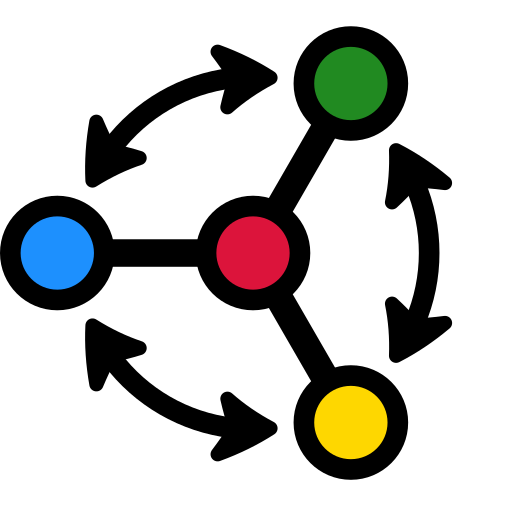
\includegraphics[height=2cm]{images/gaplogo-notext512.png}<1-> \qquad

\includegraphics[height=1.5cm]{images/2560px-RWTH_Logo_3.svg.png}<2->
\end{frame}

\begin{frame}[fragile]{Present}
\begin{itemize}
    \item<1-> GAP is still going strong \verb|(v4.15.1)| and has a large community. 
    \item<2-> It has a yearly \href{https://www.gapdays.de/gapdays2026-spring/}{conference} (This year in Portugal)
    \item<3-> It also has an yearly excellence \href{https://www.gap-system.org/award/}{awards}!
\end{itemize}
\end{frame}

\begin{frame}{What deos GAP do?}
\begin{itemize}
    \item<1-> Perform computations in group theory, ring theory, and other algebraic structures.
    \item<2-> Provide a rich library of functions for algebraic computations.
    \item<3-> Support for programming and scripting to automate tasks.
    \item<4-> Extensive documentation (\href{https://www.gap-system.org/doc}{gap-system.org/doc}) and a supportive community.
\end{itemize}
\end{frame}

\begin{frame}{Why GAP \& computation?}
\begin{itemize}
    \item<1-> Interesting groups can get BIG (Monster Group $\approx 8.08 \times 10^{53}$).
    \item<2-> Number of groups can get BIG (non-isomorphic groups of order $\leq$ 2000 (423 million groups!)).
    \item<3-> Can and has helped uncover patterns not easily seen at first.
\end{itemize}
\end{frame}


\begin{frame}{What we're going to do today?}
We're going to try to solve three group theory problems using GAP:
\begin{enumerate}
    \item<1-> Given a group, explore what we can about it.
    \item<2-> Determine if the automorphism group of a non-abelian group is also non-abelian.
    \item<3-> Conjecture trends about the commutativity ratio.
\end{enumerate}
\end{frame}


\begin{frame}{Online setup}
    We will be using \href{https://gap-online.github.io/}{mybinder} to run GAP in an online Jupyter notebook.   
    For a local setup, please refer to the \href{https://www.gap-system.org/Releases/}{GAP installation page}, but we warn this might take time. 

    \begin{quote}
        \href{https://gap-online.github.io/}{mybinder}
    \end{quote}
\end{frame}


\section{GAP as a Programming Language}
\begin{frame}[fragile]{GAP is Interpreted}
    \begin{itemize}
        \item<1-> GAP is an \textit{interpreted} language - code is executed line by line without compilation
        \item<2-> This makes it ideal for interactive exploration and rapid prototyping
        \item<3-> You can type commands directly and see results immediately
    \end{itemize}
\end{frame}

\begin{frame}[fragile]{Basic Syntax}
    GAP syntax is similar to many programming languages:
    \begin{itemize}
        \item<1-> Statements end with semicolons \verb|;| (suppress output with \verb|;;|)
        \item<2-> Comments start with \verb|#|
        \item<3-> Assignment uses \verb|:=| (not \verb|=|)
        \item<4-> Comparison uses \verb|=| for equality
        \item<5-> Comparison uses \verb|<>| for inequality
    \end{itemize}
    \pause[4]
    \begin{verbatim}
    # This is a comment
    x := 5;        # Assignment
    y := x + 3;;   # No output
    x = 5;         # Returns true
    \end{verbatim}
\end{frame}

\begin{frame}[fragile]{Lists and Indexing}
    Lists are fundamental in GAP:
    \begin{itemize}
        \item<1-> Lists are written with square brackets: \verb|[1, 2, 3]|
        \item<2-> Indexing starts at \textbf{1} (not 0!)
        \item<3-> Access elements with \verb|list[i]|
        \item<4-> List ranges: \verb|[1..10]| creates \verb|[1, 2, ..., 10]|
    \end{itemize}
    \pause[4]
    \begin{verbatim}
    mylist := [10, 20, 30];
    mylist[1];        # Returns 10
    mylist[2];        # Returns 20
    primes := [2, 3, 5, 7, 11];
    \end{verbatim}
\end{frame}

\begin{frame}[fragile]{Control Flow Keywords}
    GAP supports standard programming constructs:
    \begin{itemize}
        \item<1-> \verb|if ... then ... elif ... else ... fi|
        \item<2-> \verb|for ... in ... do ... od|
        \item<3-> \verb|while ... do ... od|
        \item<4-> \verb|function ... end|
    \end{itemize}
    \pause[4]
    \begin{verbatim}
    for i in [1..5] do
        if i mod 2 = 0 then
            Print(i, " is even\n");
        fi;
    od;
    \end{verbatim}
\end{frame}

\begin{frame}[fragile]{Functions}
    Defining functions in GAP:
    \begin{verbatim}
    square := function(x)
        return x * x;
    end;
    
    square(5);  # Returns 25
    \end{verbatim}
    \pause
    Anonymous functions with \verb|->|:
    \begin{verbatim}
    double := x -> 2 * x;
    double(7);  # Returns 14
    \end{verbatim}
\end{frame}

\begin{frame}[fragile]{Your turn}
    Write a function that computes the $n$-th Fibonacci number.
    \bigbreak
    Recall: The Fibonacci sequence is defined as:
    \begin{itemize}
        \item $F(0) = 0$
        \item $F(1) = 1$
        \item $F(n) = F(n-1) + F(n-2)$ for $n \geq 2$
    \end{itemize}
    \bigbreak
    Test your function with: \verb|Fib(10)|
\end{frame}


\section{Looking at Groups in GAP}
\begin{frame}[fragile]{Presentation of group}
    GAP provides built-in functions for a lot of known group types. These include:
    \begin{itemize}
        \item $\mathbb{Z}_n$ as \verb|CyclicGroup(n)|
        \item $S_n$ as \verb|SymmetricGroup(n)|
        \item $A_n$ as \verb|AlternatingGroup(n)|
        \item $D_n$ as \verb|DihedralGroup(2n)|
        \item Matrix Groups 
        \item Quaternion Groups 
    \end{itemize}
\end{frame}
\begin{frame}[fragile]{Presentation of group}
    Otherwise, a group can be expressed through its \textit{generators}. \\ \pause
    \verb|G := Group((1,2,3)(4,3,5));| \\ \pause
    Furthermore, any arbitrary group's elements will be represented by permutations (why?).
\end{frame}
\begin{frame}[fragile]{Analyzing a group}
    GAP can answer problems about the group and its elements. It can:
    \begin{itemize}
        \item List all the elements - \verb|Elements(G)|
        \item List all the subgroups - \verb|AllSubgroups(G)|
        \item List all the normal subgroups - \verb|NormalSubgroups(G)|
        \item Get the order of an element - \verb|Order(g)|
    \end{itemize}
\end{frame}
\begin{frame}[fragile]{Analyzing a group}
    GAP can also check if a certain property holds for a group by prepending the property with the \verb|Is| noun:
    \begin{itemize}
        \item  \verb|IsAbelian|
        \item  \verb|IsCyclic|
        \item  \verb|IsNormal|
        \item  \verb|IsIsomorphic|
    \end{itemize}
\end{frame}
\begin{frame}[fragile]{Your turn}
    Choose some group and find the following properties:
    \begin{itemize}
        \item Order
        \item Number of Conjugacy classes
        \item Order of the Largest Proper Normal Subgroup
        \item Center
        \item Exponent (google what that is)
        \item Minimal Generating set
    \end{itemize}
\end{frame}
\section{Testing Conjectures}
\begin{frame}{Testing Conjectures}
    GAP provides an easy setting to check statements and conjectures. In this section, we want to check whether the following is true or false.
    \begin{quote}
        Is the automorphism group of a non-abelian group non-abelian?
    \end{quote}
\end{frame}
\begin{frame}{Morphisms}
    In GAP, a morphism is a function between two objects of the same type (category).
    \[\operatorname{Set} \to \operatorname{Set} \]
    \[\operatorname{Grp} \to \operatorname{Grp} \]
    \[\operatorname{Ring} \to \operatorname{Ring} \]
\end{frame}
\begin{frame}[fragile]{Group Homomorphisms}
    For groups, we can define a homomorphism in two ways:
    \begin{enumerate}
        \item Defining the image of the generators.
        \item Returning a function that computes the elements.
    \end{enumerate} \pause
    We also have \verb|IsHomomorphism| to check if a function actually can be a homomorphism.
\end{frame}
\begin{frame}[fragile]{Group Automorphism}
    Automorphisms for groups follow the same rules as homomorphisms. \\\pause
    We also have \verb|AutomorphismGroup(G)| to get the automorphism group.
\end{frame}
\begin{frame}[fragile]{Your turn}
    Check our claim again.
    \begin{quote}
        Is the automorphism group of a non-abelian group non-abelian?
    \end{quote}
\end{frame}
\section{Finding Trends}
\begin{frame}{Finding Trends}
    GAP can also be great at analyzing trends and ideas.    
\end{frame}
\begin{frame}{Commutativity Ratio}
    For a finite group $G$ the probability that two group elements chosen at random with replacement commute, which we denote by $\operatorname{Pr}(G)$, is given by
    \[ \operatorname{Pr}(G) = \frac{|\{(a, b) \in G \times G \mid ab = ba\}|}{|G|^2}\]
We call $\operatorname{Pr}(G)$ the \textit{commutativity ratio} of $G$. 
\end{frame}
\begin{frame}[fragile]{Your turn}
    \begin{itemize}
        \item Compute $\operatorname{Pr}(G)$ for dihedral groups of order 6, 8, and 12
        \item Look for patterns in the results
        \item Can you conjecture a formula for $\operatorname{Pr}(G)$ in terms of the number of conjugacy classes?
    \end{itemize}
    \pause
    Hint: The number of conjugacy classes can be found using \verb|NrConjugacyClasses(G)|.
\end{frame}
\begin{frame}[fragile]{Searching All Groups}
    GAP maintains a library of all groups up to certain orders. You can search through them using:
    \begin{itemize}
        \item \verb|AllSmallGroups(n)| - Returns all groups of order $n$
        \item \verb|NumberSmallGroups(n)| - Returns the number of groups of order $n$
        \item \verb|SmallGroup(n, i)| - Returns the $i$-th group of order $n$
    \end{itemize}
    \pause
    You can also filter by properties:
    \begin{itemize}
        \item \verb|AllSmallGroups(Size, n, IsAbelian, true)|
        \item \verb|AllSmallGroups(Size, n, IsCyclic, false)|
    \end{itemize}
\end{frame}
\begin{frame}[fragile]{Your turn}
    Using the small groups library, find:
    \begin{itemize}
        \item How many non-abelian groups of order 12 exist?
        \item Which group of order 8 is the quaternion group?
        \item Find a non-cyclic group of order 15 (if it exists)
    \end{itemize}
\end{frame}
\section{Advanced Topics}
\begin{frame}[fragile]{Characters}
    GAP provides powerful tools for character theory:
    \begin{itemize}
        \item \verb|CharacterTable(G)| - Returns the character table of a group
        \item \verb|Irr(G)| - Returns the irreducible characters
        \item \verb|LinearCharacters(G)| - Returns the linear characters
    \end{itemize}
    \pause
    Character tables are useful for:
    \begin{itemize}
        \item Studying group representations
        \item Determining if groups are isomorphic
        \item Understanding conjugacy classes
    \end{itemize}
\end{frame}
\begin{frame}[fragile]{Categories}
    GAP uses categories to organize algebraic structures:
    \begin{itemize}
        \item \verb|CategoryCollections(IsObject)| - Collections of objects
        \item \verb|IsMagma| - Sets with binary operations
        \item \verb|IsSemigroup|, \verb|IsMonoid|, \verb|IsGroup| - Group-like structures
        \item \verb|IsRing|, \verb|IsField| - Ring and field structures
    \end{itemize}
    \pause
    You can check what category an object belongs to using the \verb|Is| functions.
\end{frame}
\begin{frame}[fragile]{Free Presentations}
    GAP allows you to work with groups via presentations:
    \begin{itemize}
        \item \verb|FreeGroup("a", "b")| - Creates a free group on generators
        \item \verb|/ [relator1, relator2, ...]| - Quotient by relations
    \end{itemize}
    \pause
    Example: Define $D_8 = \langle r, s \mid r^4 = s^2 = 1, srs = r^{-1} \rangle$
    \begin{verbatim}
    F := FreeGroup("r", "s");
    r := F.1; s := F.2;
    D8 := F / [r^4, s^2, s*r*s*r];
    \end{verbatim}
\end{frame}
\begin{frame}{GAP in Research}
    GAP has been instrumental in many groundbreaking mathematical discoveries:
    \begin{itemize}
        \item<1-> \textbf{Ore Conjecture (2010)}: Proved that every element of every finite non-abelian simple group is a commutator. GAP was used extensively for computational verification across thousands of groups.
        \item<2-> Classification of groups of small order
        \item<3-> Character theory computations for sporadic simple groups
        \item<4-> Verification of algebraic structures in representation theory
    \end{itemize}
    \pause[4]
    \bigbreak
    Over 3000+ papers cite GAP in their research!
\end{frame}
\begin{frame}{Further Exploration}
    Want to practice more with GAP?
    \bigbreak
    \begin{itemize}
        \item<1-> Joseph Gallian's \textit{Contemporary Abstract Algebra} includes computer exercises designed for GAP
        \item<2-> Various teaching material on the GAP website (\href{https://www.gap-system.org/doc/teach/}{gap-system.org/Teaching})
        \item<3-> Your CURIOSITY!
    \end{itemize}
\end{frame}
\begin{frame}
    \centering
    \Huge Thank You!
    \bigbreak
    \bigbreak
    \normalsize
    Questions?
    \bigbreak
    \bigbreak
    \small
    Resources: \href{https://www.gap-system.org/}{gap-system.org}
\end{frame}
\end{document}